\documentclass[11pt]{article}
\newcommand{\thetitle}{HYPERION Memo \#4: Testing the Radio Environment in 
Rangely, CO}
\newcommand{\theauthor}{Kara Kundert and Raj Biswas}
\newcommand{\theauthorsemail}{kkundert@berkeley.edu, rbiswas@berkeley.edu}
\newcommand{\thedate}{September 2017}
% the following controls some aspects of how the text is displayed on the page
\setlength{\textwidth}{6.5in}
\setlength{\textheight}{8.25in}
\setlength{\oddsidemargin}{0in}

% set up the page headers and footers
\usepackage{fancyhdr}
    \pagestyle{fancy}
    \lhead{\sffamily\slshape\small\thetitle}
    \rhead{\sffamily\small\theauthor}
    \cfoot{\sffamily\slshape\small\thepage}

% support display of graphics
\usepackage{graphicx}
\usepackage{float}

% the following control some aspects of how paragraphs are displayed
\parindent=0pt
\parskip=2ex

% import library of technical symbols
\usepackage{amsmath,amssymb,latexsym}

% import bibliography tools
\usepackage{natbib}
\citestyle{aa}

% import appendix tools
%\usepackage{appendix}

\begin{document}
% print the title in san-serif font, in bold, in huge characters
\title{
    \sffamily\bfseries\huge
    \thetitle \\
}
% print the author in san-serif font
\author{
    \sffamily\theauthor \\
    \sffamily\theauthorsemail
}
\date{\thedate}
\maketitle
\sloppy

\section{Abstract}

Radio environment is an extremely important aspect of Epoch of Reionization 
studies, as the signals are so much quieter than even most celestial sources. 
This memo aims to lay out the results of some initial radio environment testing 
in and around Rangely, Colorado. It also aims to lay out some analysis of what 
these results mean for the HYPERION instrument and suggests some new ideas for 
mitigation of environmental factors. These tests conclude that the radio 
environment around Rangely, CO makes it an ideal candidate for deployment for 
HYPERION. It also finds that local topological features can be used to 
effectively attenuate RFI signals.

\section{Background and Theory}

One aspect of the HYPERION instrument that has yet to be finalized is its 
location -- where the instrument will be deployed to do the science it is 
designed to accomplish. Since its inception, there has been frequent discussion 
of using a site near Rangely, Colorado -- a tiny town in northwestern Colorado, 
far removed from most typical sources of radio transmission and peppered with 
convenient topology. With low RFI and a somewhat quieter radio sky, it seemed 
like an ideal candidate in theory. So, we put it to the test -- what does the 
radio environment around Rangely actually look like in the HYPERION frequency 
band?  And, assuming it's a good starting point, how can we optimize it to our 
particular needs?

To answer these questions, a series of four tests were conducted: one in the 
driveway of Professor Aaron Parsons' parents house, one up a box canyon with 
limited N-EW exposure a short drive northeast, one mobile experiment with the 
antenna mounted in the back of a pick-up truck, and one in another box canyon 
with limited exposure in all directions about 15 miles southwest of Rangely.  
This changing directional exposure allowed us to begin investigating the 
effects of geological structure on the radio environment -- in particular, to 
see if rock formations around our antennas could serve as attenuators of 
ground-based sources of RFI. 

\subsection{Receiver Noise and System Temperature}

In order to determine the overall system temperature of the Rangely, CO 
deployment system, we will first need to know the receiver noise temperature, 
$T_{rx}$, i.e.  the noise that would be added at the amplifier's input in order 
to account for the added noise observed following amplification. However, it 
would be too easy for the manufacturer's to simply provide $T_{rx}$, so instead 
we'll start from a noise figure $NF$. Using Eq.~\eqref{eq:noise-figure}, we can 
calculate the noise factor $F$. For a single amplifier, we can then find the 
noise temperature using Eq.~\eqref{eq:noise-temp} with $T_0$ typically being 
set to a room temperature value of 290 K.

\begin{equation}
    \label{eq:noise-figure}
    NF = 10 \log_{10}(F)
\end{equation}

\begin{equation}
    \label{eq:noise-temp}
    F = \frac{T_0 + T}{T_0}
\end{equation}

In the case of the Rangely testing, two amplifiers were used in a chain. In 
this scenario, a final equation is needed to calculate the full receiver noise 
temperature, which accounts for the gain of the first amplifier on the effect 
of the amplifier noise contributions of the second amplifier. 

\begin{equation}
    \label{eq:receiver-temp}
    T_{rx} = T_1 + \frac{T_2}{g_1}
\end{equation}

The Rangely signal chain featured two identical amplifiers, each with a noise 
factor $NF = 11$ dB and a gain $g = 23$ dB. This led to a final receiver 
temperature of 3377 K across the band.

As discussed in~\citet{kundert2016}, we would  like for our overall system 
temperature $T_{sys} = T_{rx} + T_{sync}$ to be dominated by a known term, such 
as the galactic synchrotron emission, $T_{sync}$, which can be calculated using 
Eq.~\eqref{eq:sync-temp} using a value of $\beta = 2.5$.

\begin{equation}
    \label{eq:sync-temp}
    T_{sync}(\nu) = T_{sync}(\nu = \textrm{150 MHz}) 
    \left(\frac{\nu}{\textrm{150 MHz}}\right)^{-\beta}
\end{equation}

With the receiver temperature calculated in Eq.~\eqref{eq:receiver-temp} and 
the sky temperature calculated with Eq.~\eqref{eq:sync-temp}, we can find the 
difference between the total system temperature and the known sky temperature 
using Eq.~\eqref{eq:dB-to-sky}.

\begin{equation}
    \label{eq:dB-to-sky}
    \textrm{dB} = 10 \log\left(\frac{T_{sys}}{T_{sync}}\right)
\end{equation}

From this, we find that the system temperature $T_{sys}$ is approximately 5 dB 
brighter than the sky temperature $T_{sync}$ at 70 MHz, as can be seen in 
Fig.~\ref{fig:noise-floor}.  This indicates that the receiver system used 
during this round of testing will be inadequate for observations, as it will be 
difficult to properly calibrate the system with such a high level of noise 
being generated by our system.

\begin{figure}
    \begin{center}
    \includegraphics[width=\linewidth]{/home/kara/src/python/berkeley/plotters/noise_floor_rangely.png}
    \end{center}
    \caption{
        In this figure, we can see how the receiver temperature contributed to 
        the overall system. Ideally, we would like to be able to lower the 
        system temperature to the point where the synchrotron sky is the main 
        term across the band. However, as is evident above, the receiver chain 
        used in this particular testing trip introduced about 3400 K in noise 
        temperature, drowning out all but the absolute lowest frequencies of 
        the synchrotron sky. All in all, the synchrotron sky is approximately 5 
        dB down from the overall system temperature at 70 MHz.  In future 
        testing, we will need to develop a lower temperature signal chain to 
        mitigate this effect.
    }
    \label{fig:noise-floor}
\end{figure}

\section{Method}

In each of these tests, a broadband dipole was hooked up to the FieldFox 
spectrum analyzer and used to record all that it picked up in a given frequency 
band (either 80-110 MHz or 0-300 MHz). Each spectra held 1001 points and was 
averaged for approximately 1 minute, collecting a maximum, minimum, and average 
spectrum for each recording.

In the first experiment, the observations were taken in the driveway at 
Professor Parsons' parents' house. There was an RFI source around 193.5 MHz, 
which was assumed to be emitted from the nearby oilfield towards NE. So, the 
observations were done with on-axis (i.e. in the beam null) and off-axis (i.e.  
in the beam peak) alignment of the antenna with respect to the oilfield.

In the second experiment, measurements were taken up the canyon where the
place was shielded by the landscape towards the north, east, and west (with a 
horizon altitude of $57^{\circ}$ to the W). The southern direction was most 
exposed, with a horizon altitude of only $4^{\circ}$ degrees.

In the third experiment, the antenna was mounted onto the back of a pickup 
truck and observations were taken at various locations, starting at the house 
and ending well up Cottonwood Canyon.

Finally, after traveling up Cottonwood Canyon into a shallow box canyon, the 
antenna was dismounted from the truck and placed in a creek bed with rock walls 
raising the horizon in all directions. There, observations were taken in both 
frequency bands in both E-W and N-S dipole orientations.

\section{Data and Analysis}

Rangely, Colorado is already an attractive candidate for low-frequency radio 
astronomy, as there are only a handful of known emitters in the FM band. As can 
be seen in Fig.~\ref{fig:102}, even when standing in the driveway of Professor 
Parsons' parents' house, there's only about 13 visible sources of RFI within 
the HYPERION science band and all have a maximum amplitude of less than -20 
dBm. However, by being strategic, we can get even better results.

Table~\ref{tab:rfi-sources} shows the visible FM sources from the box canyon up 
Cottonwood Canyon, the site we found to have the minimum amount of RFI 
contamination. At a maximum, these five FM stations have a power level of -50 
dBm. These kinds of contamination rates make Rangely, CO competitive with other 
hallmark radio observatory sites, such as the Karoo Desert in South Africa.

\begin{center}
 \begin{tabular}{ |c|c|c| }
  \hline
  FM station & Frequency(MHz) & Power Level (dBm) \\
  \hline
  KXRQ Roosevelt & 94.3  & -50 \\
  \hline
  KIFX Vernal    & 98.5  & -50 \\
  \hline
  KCUA Naples    & 92.5  & -57 \\
  \hline
  (Undefined)    & 106.4 & -57 \\
  \hline
  KMZK Clifton   & 106.9 & -57 \\
  \hline
  \end{tabular}
  \label{tab:rfi-sources}
\end{center}

Moreover, our data indicates that local topology can have a strong effect on 
the visibility and strength of RFI sources. In comparing Figs.~\ref{fig:103} 
and~\ref{fig:104}, we see that in changing the orientation of the antenna and 
therefore the beam relative to the point of maximum exposure in the south, we 
change the what RFI sources are seen and their amplitudes. More exposure 
translates to more visible sources and more power in that direction.

This has huge consequences to HYPERION, which is built upon our ability to 
modify the ``horizon" of the sky using absorbers to impose an artificially tall 
horizon and force the sky into higher order spatial Fourier modes. The effects 
of these rock faces in these initial results shows that it's possible to 
generate this kind of effect naturally by using local geological structures to 
our advantage. While these natural structures won't replace our need for 
high-performance, low-frequency absorber entirely, they could help attenuate 
the bright galactic sky signal in those directions and therefore lower our 
overall system temperature.

\section{Conclusions}

In this round of field testing, we hoped to gain some insight into the overall 
RFI environment of Rangely, CO and to learn whether it would be a good 
candidate site for the HYPERION experiment. The data acquired is very 
promising, indicating that even the worst conditions (those in the driveway of 
Professor Parsons' parents' house) in Rangely are pretty clean for our 
purposes.  Moreover, the best conditions (those from the secluded box canyon to 
the southwest) are superior to even those in the nationally protected radio 
reserves in the Karoo Desert in South Africa.

One remarkable feature observed in the data is the strong effect that local 
topology can have on our observations and RFI environment. In limiting our 
exposure to different directions using naturally occurring geological features, 
we were able to reduce the number of visible RFI sources from approximately 13  
with amplitudes between -60 and -20 dBm to only two with amplitudes below -45 
dBm.  That's a very strong and valuable effect, and one that is unique to the 
geology in the area.

While there is still quite a bit that would need to be determined before 
planning a deployment in CO, this site remains our best candidate for the final 
HYPERION experiment.

\bibliography{hyperion}{}
\bibliographystyle{apj}

\appendix

\section{Data from Driveway Observations}

\begin{figure}[H]
 \begin{center}
 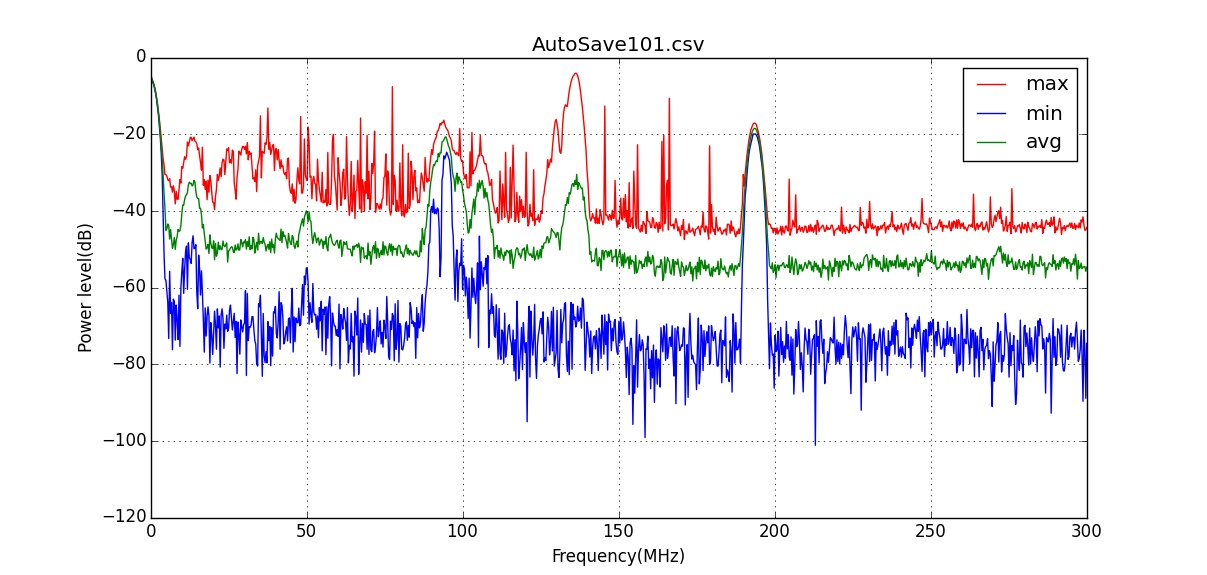
\includegraphics[width=\linewidth]{/home/kara/documents/hyperion/memos/memo4/plots/101.jpeg}
 \end{center}
 \caption{
        Pictured above is the radio environment from 0-300 MHz as measured from 
        the driveway of Professor Parsons' parents' house, with the antenna 
        axis aligned with the oilfield in the northeast. This puts the oilfield 
        transmission at 193.5 MHz in the null of the beam.
 }
 \label{fig:101}
\end{figure}

\begin{figure}[H]
 \begin{center}
 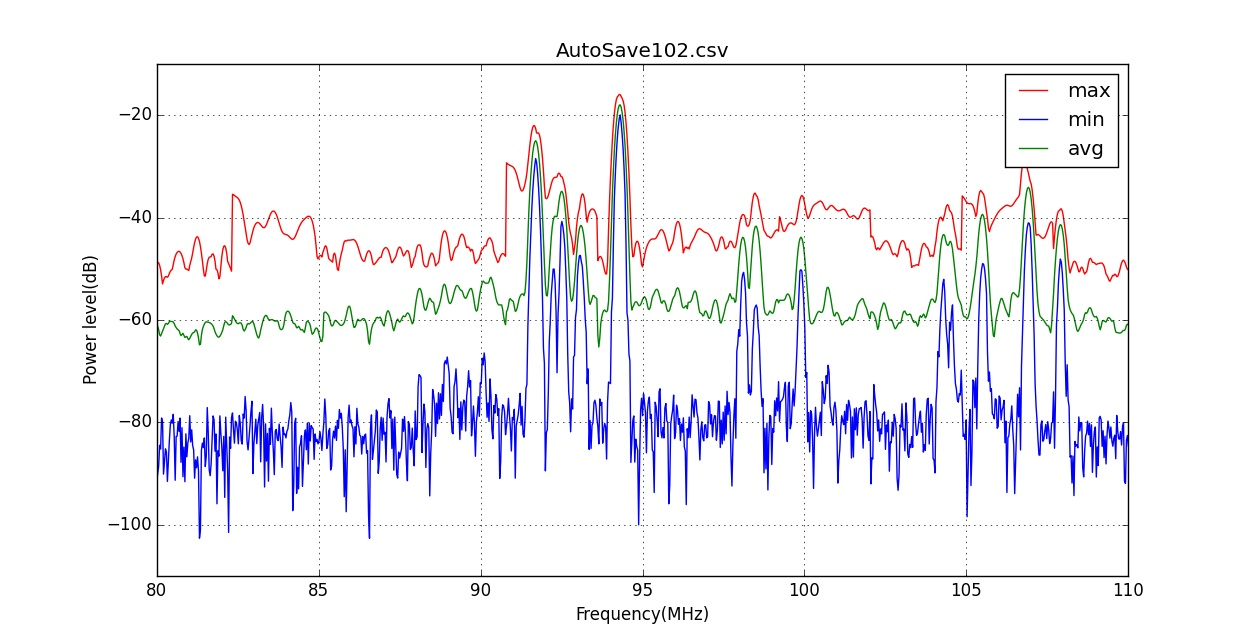
\includegraphics[width=\linewidth]{/home/kara/documents/hyperion/memos/memo4/plots/102.jpeg}
 \end{center}
 \caption{
        Pictured above is the radio environment from 80-110 MHz as measured 
        from the driveway of Professor Parsons' parents' house. As can be 
        easily seen, there are approximately 13 unique and strong sources of 
        RFI with amplitudes between -60 and -20 dBm.
 }
 \label{fig:102}
\end{figure}

\section{Data from Northeastern Box Canyon}

\begin{figure}[H]
 \begin{center}
 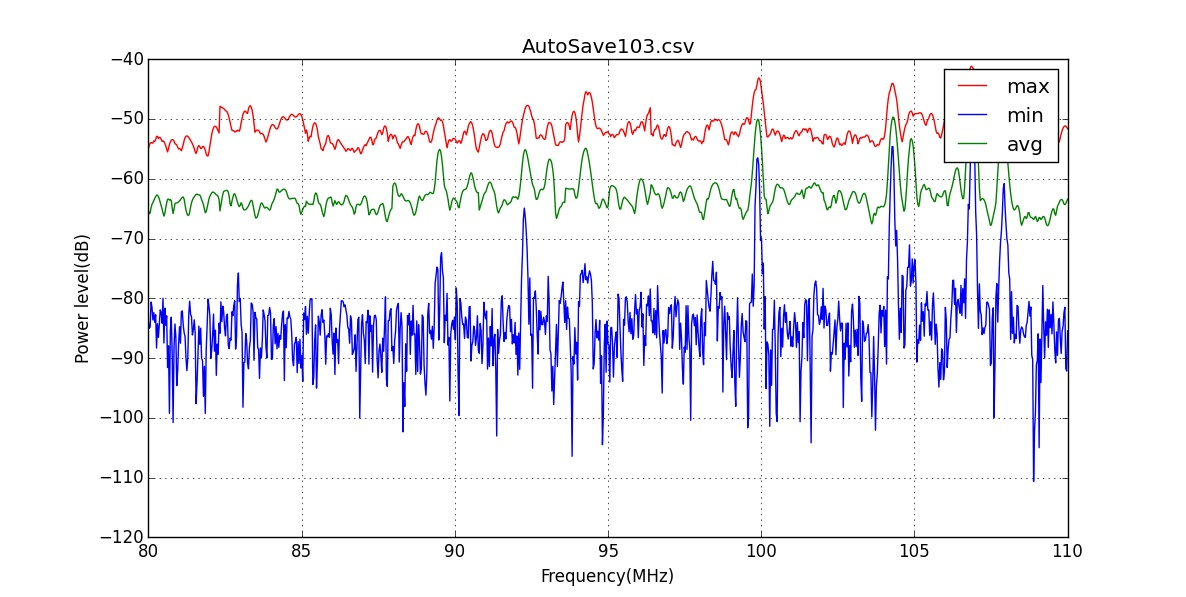
\includegraphics[width=\linewidth]{/home/kara/documents/hyperion/memos/memo4/plots/103.jpeg}
 \end{center}
 \caption{
        Pictured above is the radio environment from 80-110 MHz as measured 
        from a box canyon to the northeast of the house, with the dipole axis 
        aligned N-S. This alignment points the null of the antenna beam towards 
        the point of the lowest horizon altitude ($4^{\circ}$), and the peak of 
        the beam towards the most geologically sheltered part of the canyon.  
        Already much of the RFI from the environment has been strongly 
        attenuated, and there are only five remaining sources with amplitudes 
        between -70 and -45 dBm.
 }
 \label{fig:103}
\end{figure}

\begin{figure}[H]
 \begin{center}
 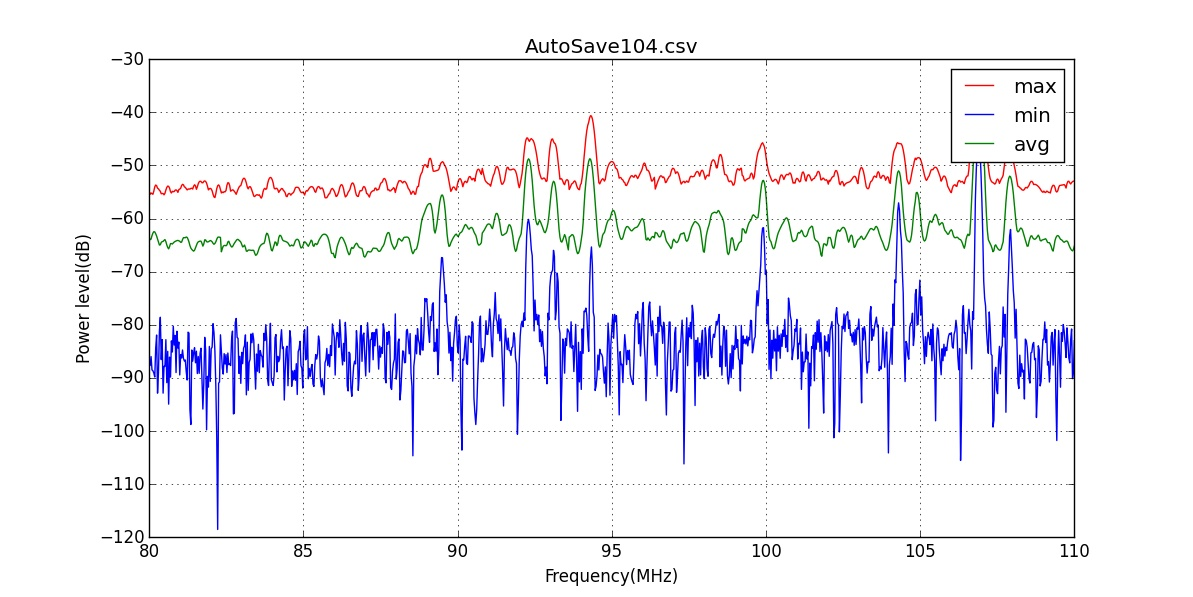
\includegraphics[width=\linewidth]{/home/kara/documents/hyperion/memos/memo4/plots/104.jpeg}
 \end{center}
 \caption{
        Pictured above is the radio environment from 80-110 MHz as measured 
        from a box canyon to the northeast of the house, with the dipole axis 
        aligned E-W. This alignment points the peak of the antenna beam towards 
        the point of the lowest horizon altitude ($4^{\circ}$), and the null of 
        the beam towards the most geologically sheltered part of the canyon.  
        This arrangement is visibly worse than the previous one, with eight 
        sources of RFI now visible in the spectra with amplitudes between -70 
        and -35 dBm.
 }
 \label{fig:104}
\end{figure}

\begin{figure}[H]
 \begin{center}
 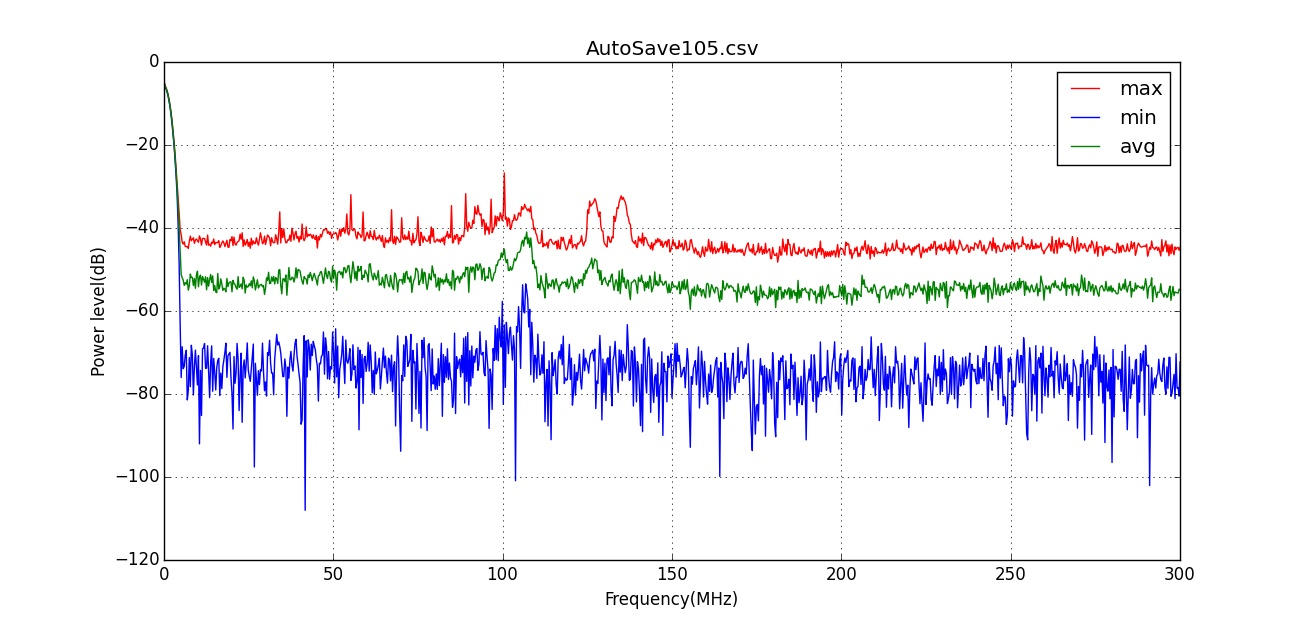
\includegraphics[width=\linewidth]{/home/kara/documents/hyperion/memos/memo4/plots/105.jpeg}
 \end{center}
 \caption{
        Pictured above is the radio environment from 0-300 MHz as measured from 
        a box canyon to the northeast of the house, with the dipole axis 
        aligned N-S. This alignment points the null of the antenna beam towards 
        the point of the lowest horizon altitude ($4^{\circ}$), and the peak of 
        the beam towards the most geologically sheltered part of the canyon.  
        Most of the RFI contamination is contained within the FM band, with no 
        strong signals appearing beyond approximately 140 MHz. All sources of 
        RFI have an amplitude of less than -25 dBm, and there are two new 
        bright sources with peaks around 125 MHz and 135 MHz.
 }
 \label{fig:105}
\end{figure}


\begin{figure}[H]
 \begin{center}
 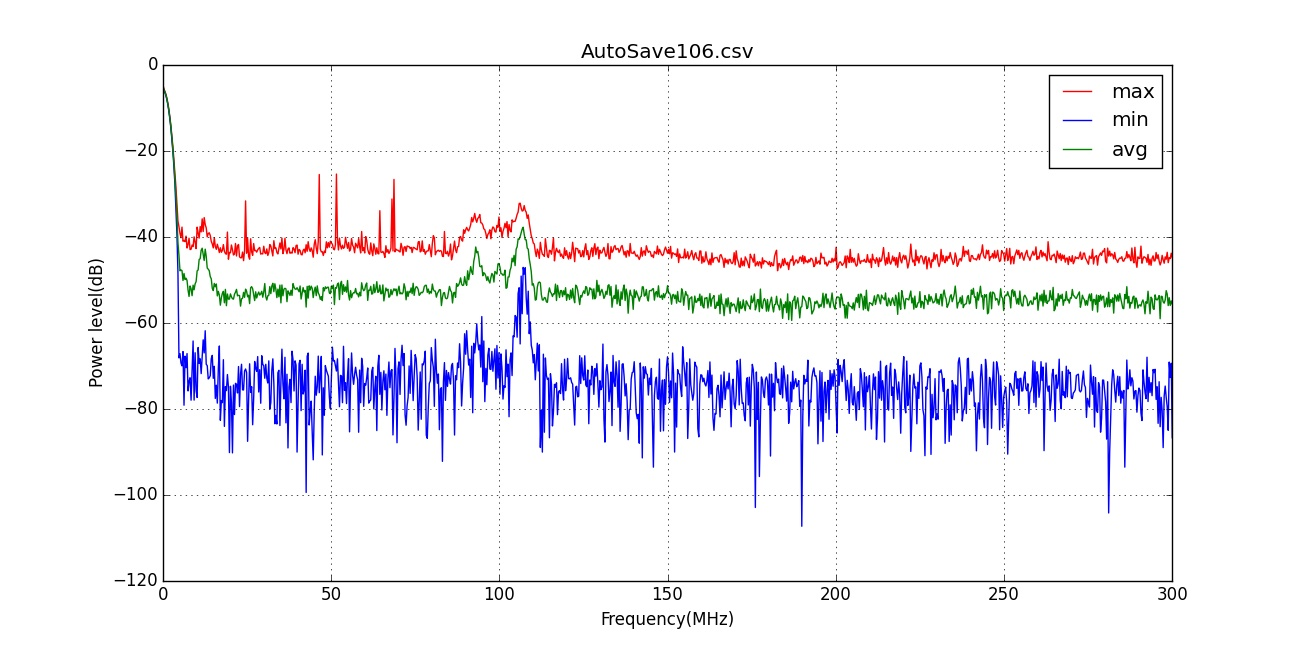
\includegraphics[width=\linewidth]{/home/kara/documents/hyperion/memos/memo4/plots/106.jpeg}
 \end{center}
 \caption{
        Pictured above is the radio environment from 0-300 MHz as measured from 
        a box canyon to the northeast of the house, with the dipole axis 
        aligned E-W. This alignment points the peak of the antenna beam towards 
        the point of the lowest horizon altitude ($4^{\circ}$), and the null of 
        the beam towards the most geologically sheltered part of the canyon.  
        Most of the RFI contamination is contained within the FM band, with no 
        strong signals appearing beyond approximately 110 MHz. All sources of 
        RFI have an amplitude of less than -25 dBm, though the ones that are 
        present have higher power levels than in the N-S alignment. The sources 
        seen at 125 and 135 MHz are no longer visible, indicating that they 
        were being transmitted from somewhere in the E-W directions of the 
        canyon.
 }
 \label{fig:106}
\end{figure}

\section{Data from Mounted Truck Observations}

\begin{figure}[H]
    \begin{center}
    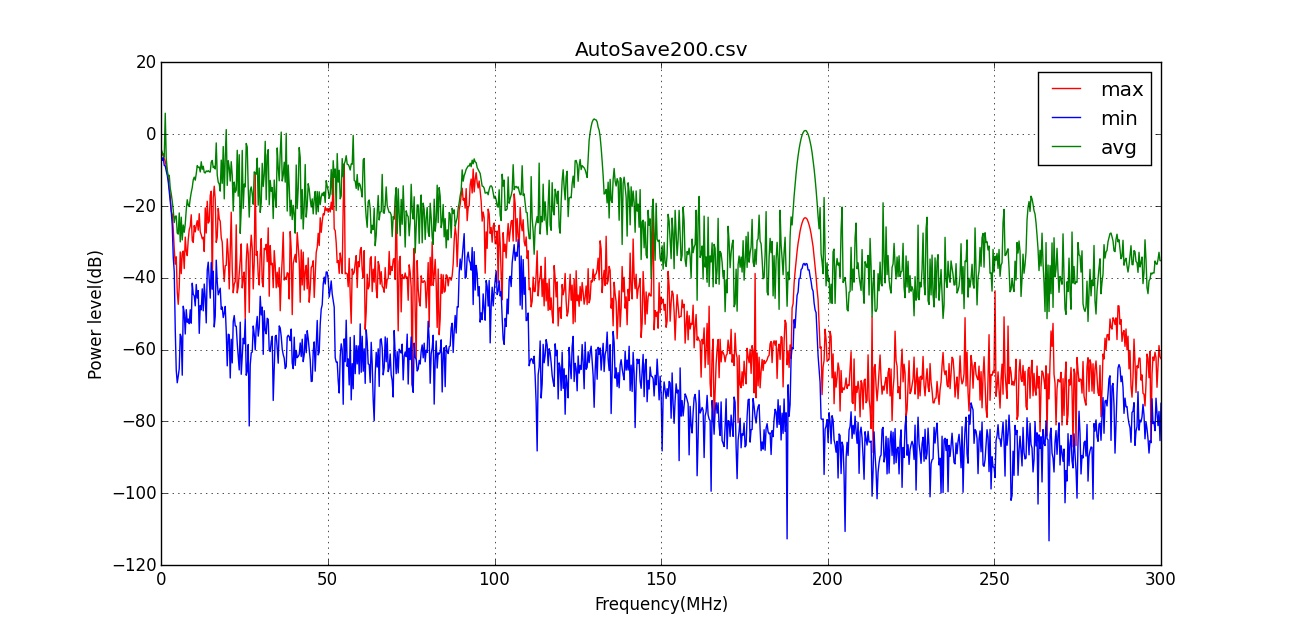
\includegraphics[width=\linewidth]{/home/kara/documents/hyperion/memos/memo4/plots/200.jpeg}
    \end{center}
    \caption{
        Pictured above is the radio environment from 0-300 MHz as measured from 
        the house, with the dipole mounted in the back of a pick-up truck.  
        This arrangement, while convenient for mobility, clearly introduces a 
        fair amount of reflections and other spectral features. The strongest 
        RFI sources in this spectrum have amplitudes of more than 0 dBm and a 
        maximum noise floor ranging between -40 and -20 dBm, making this the 
        loudest and noisiest spectrum measured in this set of experiments.
    }
    \label{fig:200}
\end{figure}

\begin{figure}[H]
    \begin{center}
    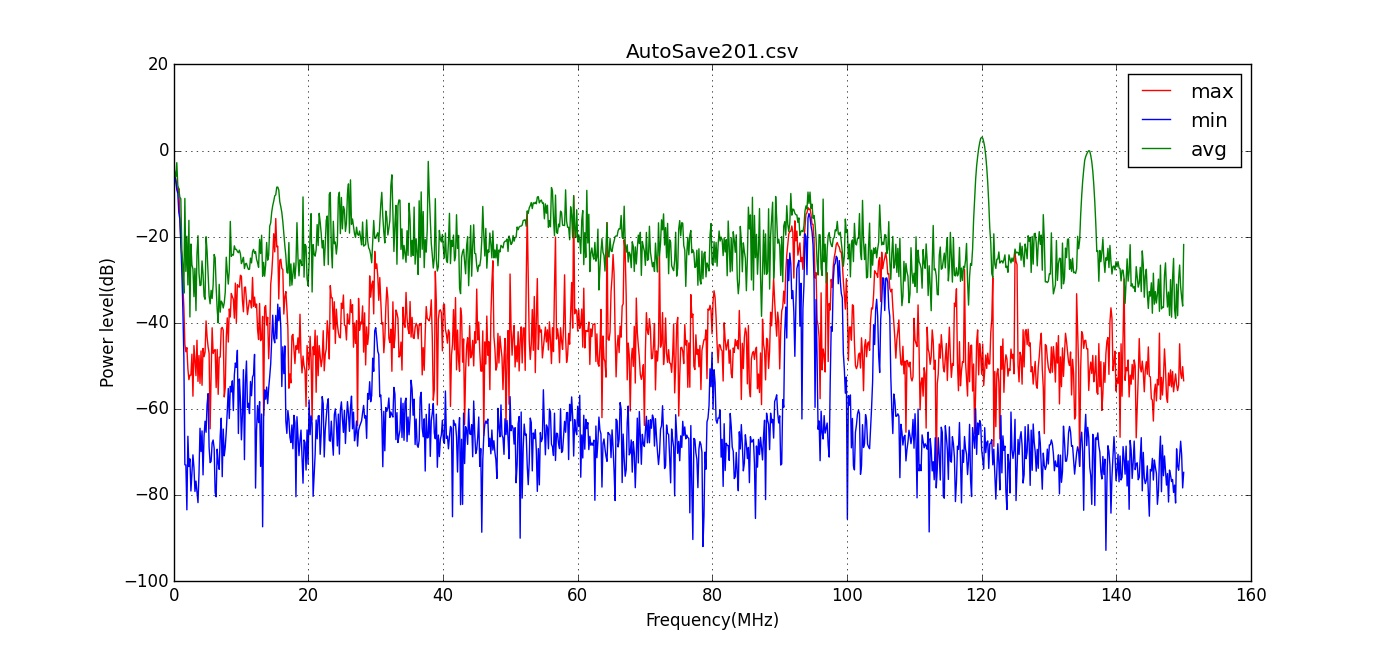
\includegraphics[width=\linewidth]{/home/kara/documents/hyperion/memos/memo4/plots/201.jpeg}
    \end{center}
    \caption{
        Pictured above is the radio environment from 0-150 MHz as measured from 
        City Road 2, with the dipole mounted in the back of a pick-up truck.  
        The strongest RFI sources in this spectrum have amplitudes of more than 
        0 dBm and a maximum noise floor ranging between -30 and -20 dBm, making 
          this a marginally better spectrum than the data set shown in the 
          previous figure.
    }
    \label{fig:201}
\end{figure}
\begin{figure}[H]
    \begin{center}
    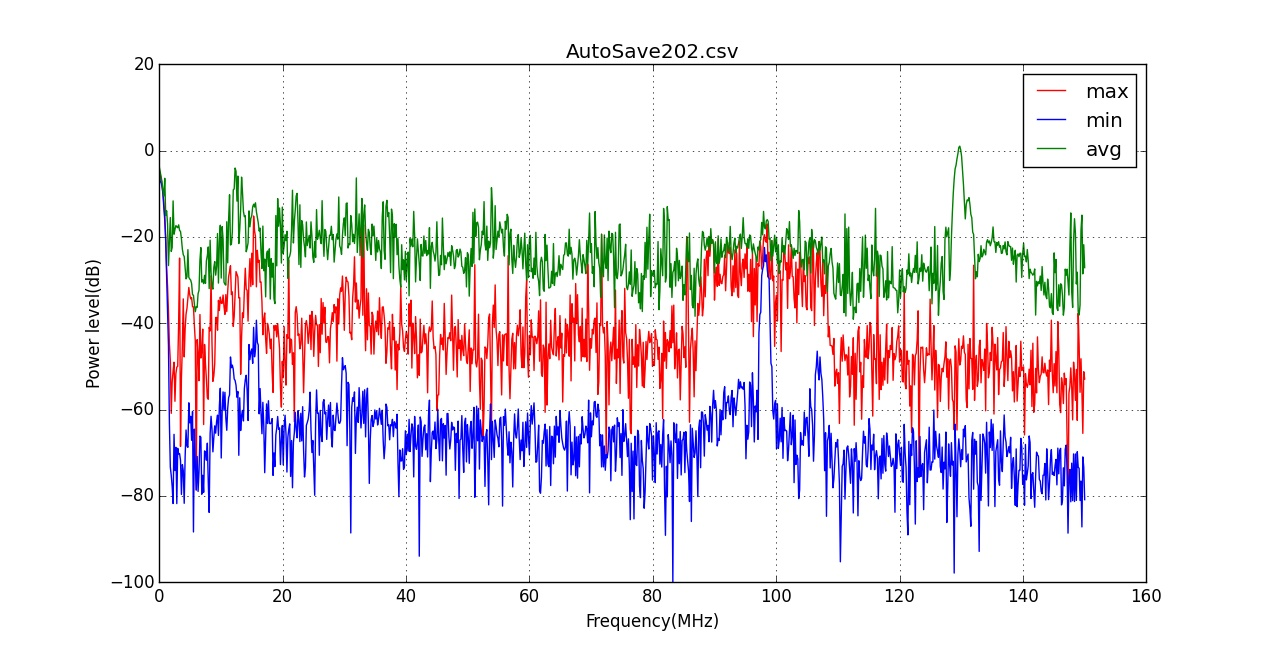
\includegraphics[width=\linewidth]{/home/kara/documents/hyperion/memos/memo4/plots/202.jpeg}
    \end{center}
    \caption{
        NOTE: I CAN'T READ THESE NOTES, I DON'T KNOW WHAT THIS MEASUREMENT IS
    }
    \label{fig:202}
\end{figure}
\begin{figure}[H]
    \begin{center}
    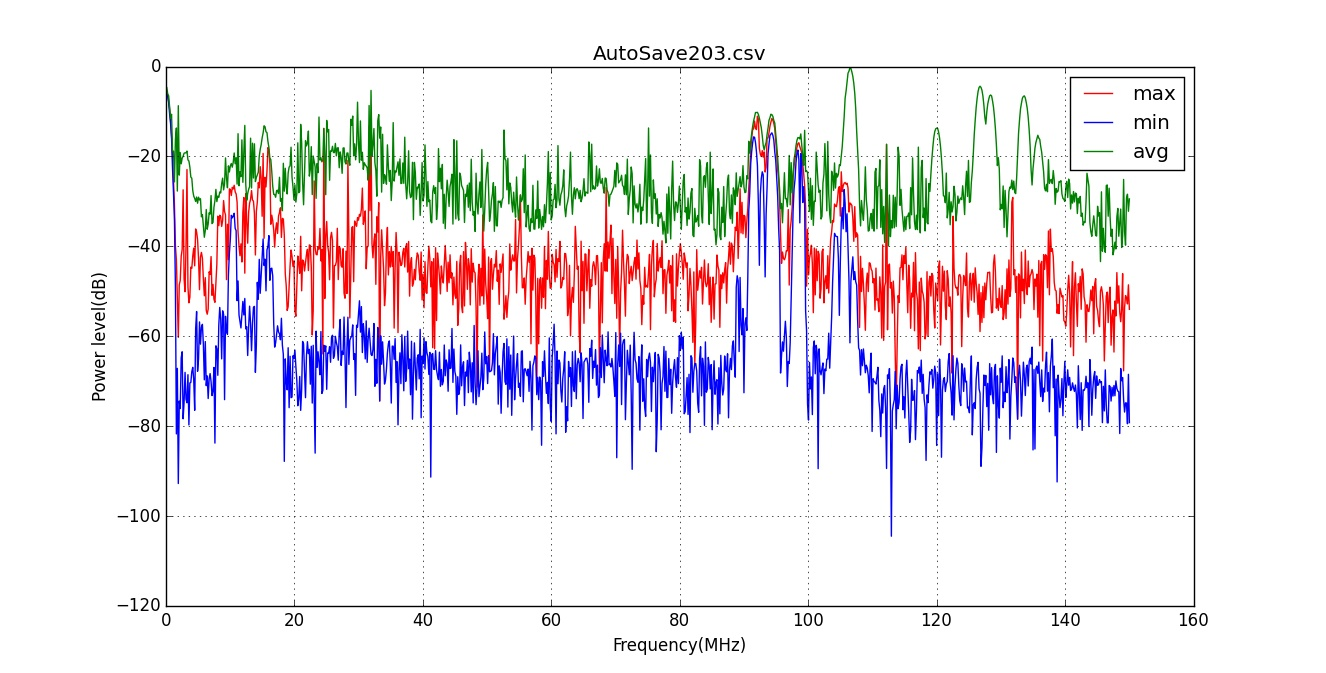
\includegraphics[width=\linewidth]{/home/kara/documents/hyperion/memos/memo4/plots/203.jpeg}
    \end{center}
    \caption{
        Pictured above is the radio environment from 0-150 MHz as measured from 
        a shallow hollow at the entrance to Cottonwood Canyon, with the dipole 
        mounted in the back of a pick-up truck.  The spectrum has a maximum 
        noise floor ranging between -30 and -20 dBm, and approximately seven 
        consistent sources of RFI between 90-110 MHz. Most of the higher 
        frequency RFI sources between 120-138 MHz appear to be transient, only 
        appearing in the maximum spectrum and not the average or minimum 
        spectra. All RFI sources have an amplitude of less than 0 dBm in this 
        observation, and the consistent sources only have a max amplitude of 
        approximately -10 dBm. Even in this very noisy data set, it's already 
        apparent that Cottonwood Canyon could be a promising deployment site.
        NOTE: ALSO STRUGGLING TO READ THIS
    }
    \label{fig:203}
\end{figure}
\begin{figure}[H]
    \begin{center}
    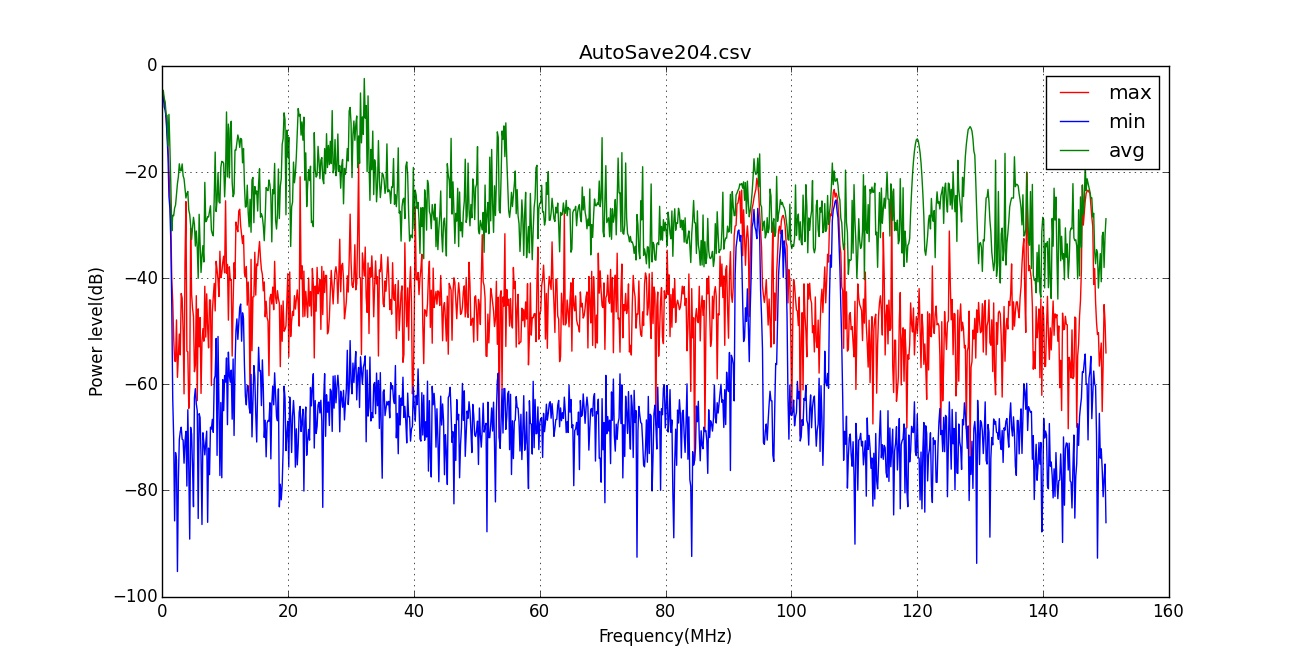
\includegraphics[width=\linewidth]{/home/kara/documents/hyperion/memos/memo4/plots/204.jpeg}
    \end{center}
    \caption{
        Pictured above is the radio environment from 0-150 MHz as measured from 
        three miles up the road into Cottonwood Canyon, with the dipole mounted 
        in the back of a pick-up truck.  The spectrum has a maximum noise floor 
        ranging between -30 and -20 dBm, and approximately four consistent 
        sources of RFI between 90-110 MHz. Most of the higher frequency RFI 
        sources between 120-138 MHz appear to be transient, only appearing in 
        the maximum spectrum and not the average or minimum spectra. All RFI 
        sources have an amplitude of less than -10 dBm in this observation, and 
        the consistent sources only have a max amplitude of approximately -25 
        dBm. Going deeper into the canyon and using the shallow rock walls as 
        natural attenuators to local RFI is proving to be an effective method.
    }
    \label{fig:204}
\end{figure}
\begin{figure}[H]
    \begin{center}
    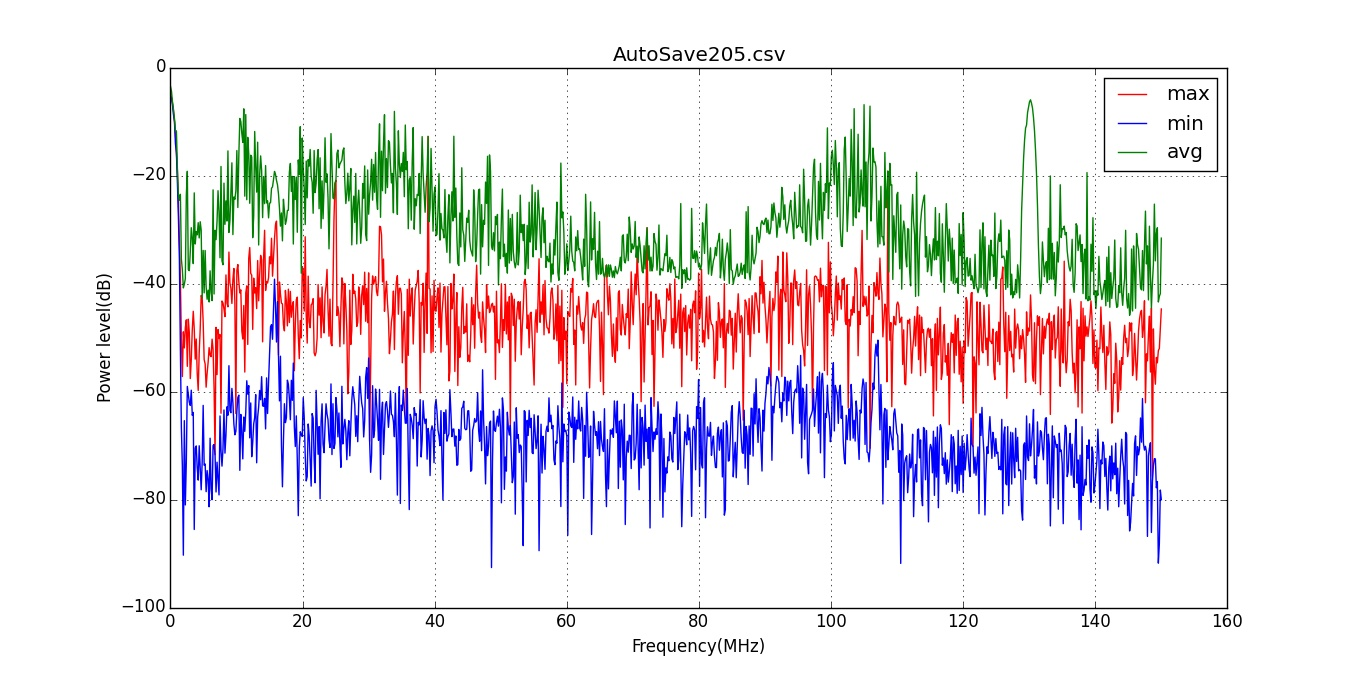
\includegraphics[width=\linewidth]{/home/kara/documents/hyperion/memos/memo4/plots/205.jpeg}
    \end{center}
    \caption{
        Pictured above is the radio environment from 0-150 MHz as measured from 
        a small box canyon approximately five miles up the road into Cottonwood 
        Canyon, with the dipole mounted in the back of a pick-up truck.  The 
        spectrum has a maximum noise floor ranging between -40 and -20 dBm, an 
        average noise floor of -45 dBm, and no visible consistent sources of 
        RFI.  There is one higher frequency RFI source centered at 130 MHz that 
        appears to be transient, only appearing in the maximum spectrum and not 
        the average or minimum spectra, with an amplitude of approximately -10 
        dBm.  This is the best candidate site yet, and is further explored in 
        the next round of testing upon being removed from the back of the 
        truck.
    }
    \label{fig:205}
\end{figure}

\section{Data from Cottonwood Road Box Canyon}

\begin{figure}[H]
    \begin{center}
    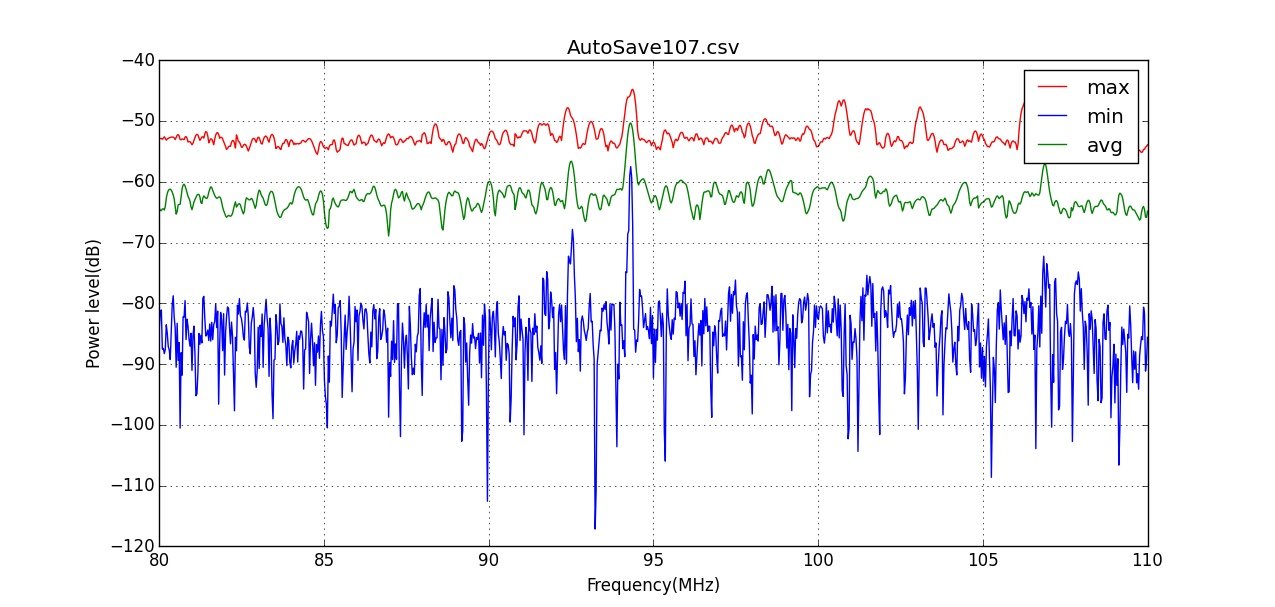
\includegraphics[width=\linewidth]{/home/kara/documents/hyperion/memos/memo4/plots/107.jpeg}
    \end{center}
    \caption{
        Pictured above is the radio environment from 80-110 MHz as measured 
        from the creek bed in the box canyon off of Cottonwood Road, 
        approximately 15 miles southwest of Rangely, with the dipole axis 
        aligned E-W.  This is the cleanest radio sky that we observed, with 
        only two visible sources of RFI and both with amplitudes of less than 
        -45 dBm.  This was also the most sheltered testing location, where the 
        box canyon had faces on all sides of the antenna.
    }
    \label{fig:107}
\end{figure}

\begin{figure}[H]
    \begin{center}
    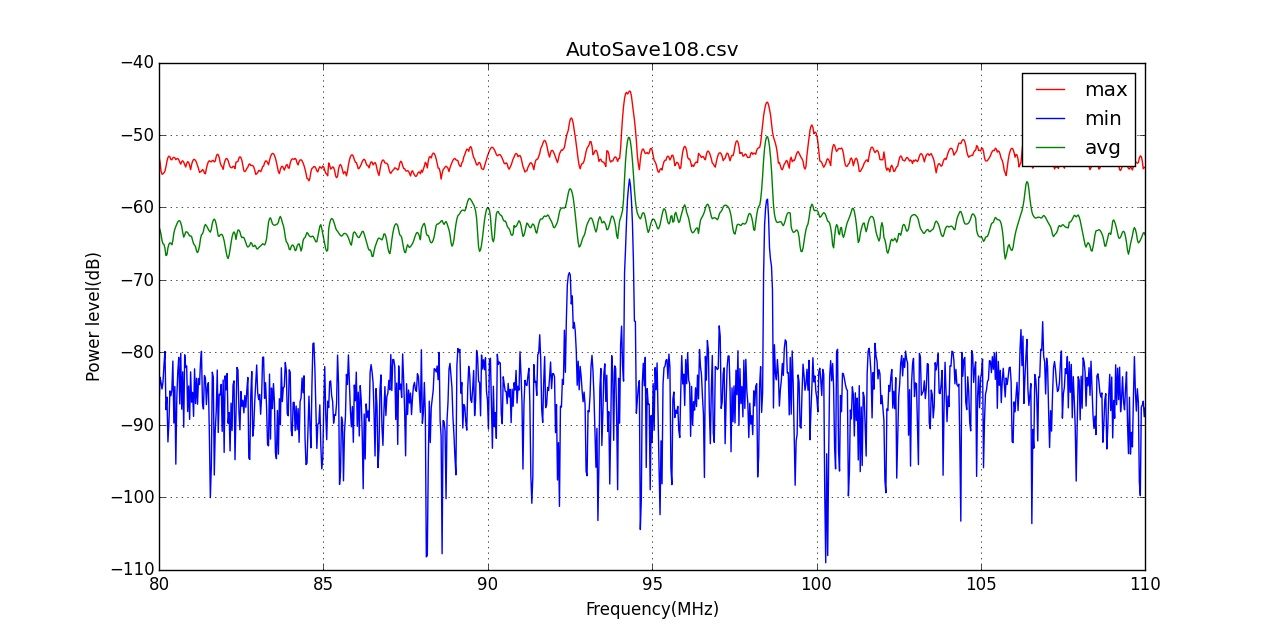
\includegraphics[width=\linewidth]{/home/kara/documents/hyperion/memos/memo4/plots/108.jpeg}
    \end{center}
    \caption{
        Pictured above is the radio environment from 80-110 MHz as measured 
        from the creek bed in the box canyon off of Cottonwood Road, 
        approximately 15 miles southwest of Rangely, with the dipole axis 
        aligned N-S.  Although not quite as impeccable as the previous figure, 
        there are still only three visible sources of RFI in this spectra and 
        all have amplitudes of less than -45 dBm.
    }
    \label{fig:108}
\end{figure}

\begin{figure}[H]
    \begin{center}
    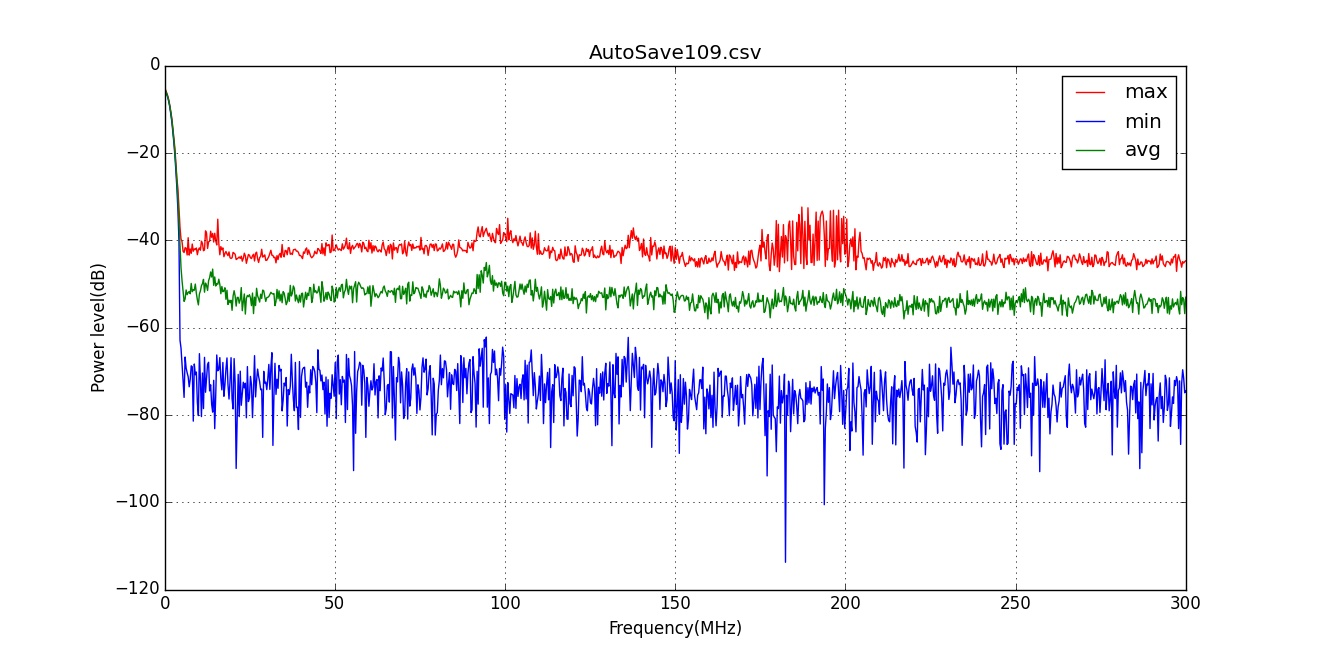
\includegraphics[width=\linewidth]{/home/kara/documents/hyperion/memos/memo4/plots/109.jpeg}
    \end{center}
    \caption{
        Pictured above is the radio environment from 0-300 MHz as measured from 
        the creek bed in the box canyon off of Cottonwood Road, approximately 
        15 miles southwest of Rangely, with the dipole axis aligned E-W.  
           Overall, this is a very clean radio sky, with some fuzz appearing 
           intermittently between 175-205 MHz. We believe this originates from 
           the local oilfields. This was also the most sheltered testing 
           location, where the box canyon had faces on all sides of the 
           antenna.
    }
    \label{fig:109}
\end{figure}

\begin{figure}[H]
    \begin{center}
    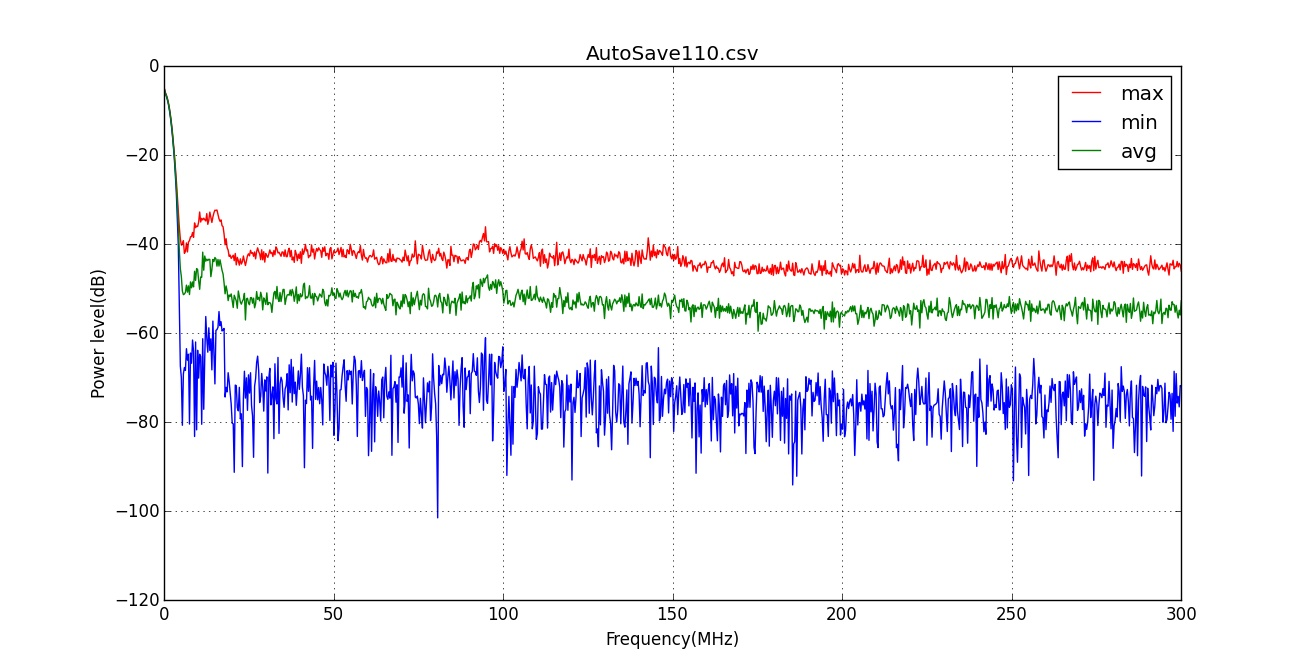
\includegraphics[width=\linewidth]{/home/kara/documents/hyperion/memos/memo4/plots/110.jpeg}
    \end{center}
    \caption{
        Pictured above is the radio environment from 0-300 MHz as measured from 
        the creek bed in the box canyon off of Cottonwood Road, approximately 
        15 miles southwest of Rangely, with the dipole axis aligned N-S. All 
           RFI sources are very attenuated here, and the high frequency fuzz 
           seen between 175-205 MHz in the previous figure is no longer 
           visible, as the oilfields are now in the null of the dipole beam.
    }
    \label{fig:110}
\end{figure}

\end{document}
